%%%%%%%%%%%%%%%%%%%%%%%%%%%%%%%%%%%%%%%%%%%%%%%%%%%%%%%%%%%%%%%%%%%
%%% Documento LaTeX 																						%%%
%%%%%%%%%%%%%%%%%%%%%%%%%%%%%%%%%%%%%%%%%%%%%%%%%%%%%%%%%%%%%%%%%%%
% Título:		Capítulo 1
% Autor:  	Ignacio Moreno Doblas
% Fecha:  	2014-02-01
% Versión:	0.5.0
%%%%%%%%%%%%%%%%%%%%%%%%%%%%%%%%%%%%%%%%%%%%%%%%%%%%%%%%%%%%%%%%%%%
\chapterbegin{Introducción teórica}
%\minitoc

%\begin{sinopsis}
%\label{sec:chpltx:sinop}
%	
%\end{sinopsis}

\section{Bluetooth}
\label{sec:Bluetooth}


\subsection{Historia}

	En 1994 Ericsson inició un estudio para investigar la viabilidad de un sistema de comunicaciones vía radio, de bajo coste y bajo consumo, para la interconexión entre teléfonos móviles y otros accesorios con la intención de eliminar cables entre aparatos. El estudio partía de un largo proyecto que investigaba sobre unos dispositivos transceptores conectados a una red celular, hasta llegar a un enlace de radio de corto alcance, llamado \tit{MC link}.

	Conforme este proyecto avanzaba, se empezó a visualizar que este tipo de enlace podía ser utilizado ampliamente en un gran número de aplicaciones, ya que tenía como principal virtud el basarse en un chip de radio relativamente económico. 
 
	A comienzos de 1997, según avanzaba el proyecto \tit{MC link}, Ericsson fue despertando el interés de otros fabricantes de equipos portátiles. De seguida se vio claramente que para que el sistema tuviera éxito un gran número de equipos deberían estar equipados con esta tecnología. Esto fue lo que llevó, a principios de 1998, a crear un \ac{SIG}, formado por 5 promotores que eran: Ericsson, Nokia, IBM, Toshiba e Intel. La idea era lograr un conjunto adecuado de áreas de negocio, dos líderes del mercado de las telecomunicaciones, dos líderes del mercado de los ordenadores portátiles y un líder de la fabricación de chips. A día de hoy hay más de 20.000 empresas que lo conforman.

	Obviamente Bluetooth no se llamó así desde un comienzo. El origen surge en 1994, cuando uno de los desarrolladores, Jim Kardach, propuso el nombre de uno de los reyes vikingos, específicamente el de Harald Blåtand, cuya traducción al inglés es Harald Bluetooth.
	
	Este rey fue conocido por unificar las tribus noruegas, suecas-danesas y por convertirlas al cristianismo, que en paralelo es la fusión de la comunicación de los sistemas digitales, que buscaba reemplazar el cable para los dispositivos móviles.
	

\begin{figure}[h] \centering
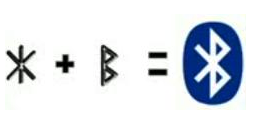
\includegraphics[width=6cm]{graphs/bluetooth_logo.png} 
\caption{Origen del logotipo comercial de Bluetooth \cite{bluetoothoficial}}
\label{bluetoothOrigin}
\end{figure}

	Aún hay más misterios escandinavos relacionados con la tecnología como cuál es el origen del logotipo. El logotipo es una combinación de dos letras del alfabeto rúnico, precisamente la H y la B. Dicha fusión se aprecia en la figura \ref{bluetoothOrigin}.

\subsection{Usos y aplicaciones }\label{cap:usosAplicaciones}
	Se denomina Bluetooth a la norma que define un estándar global de comunicación inalámbrica, que posibilita la transmisión de voz y datos entre diferentes equipos mediante un enlace por radiofrecuencia. Los principales objetivos que se pretende conseguir con esta norma son: facilitar las comunicaciones entre equipos móviles y fijos, eliminar cables y conectores entre estos, ofreciendo la posibilidad de crear pequeñas redes inalámbricas y facilitar la sincronización de datos entre nuestros equipos personales.
	
	Los dispositivos que incorporan este protocolo pueden comunicarse entre sí cuando se encuentran dentro de su radio de alcance. Las comunicaciones se realizan por radiofrecuencia de forma que los dispositivos no tienen que estar alineados y pueden incluso estar en habitaciones separadas si la potencia de transmisión es suficiente. Estos dispositivos se clasifican como Clase 1, Clase 2 o Clase 3 en referencia a su potencia de transmisión, tal y como muestra la tabla \ref{bluetoothTable}

\begin{table}[H]%
	\centering
\begin{tabular}{|c|c|c|c|}
	\hline
	\hline
	\tbf{Clase}&\tbf{\specialcell{Potencia máxima \\ permitida (mW)}} &\tbf{\specialcell{Potencia máxima \\ permitida (dBm)}}&\tbf{\specialcell{Alcance \\ (aproximado)}}\\ \hline 
	\tbf{Clase 1}&100 mW&20 dBm&100 metros\\ \hline
	\tbf{Clase 2}&2.5 mW&4 dBm&5-10 metros\\ \hline
	\tbf{Clase 3}&1 mW&0 dBm&1 metro\\ \hline
	\hline 
\end{tabular}
\caption{Clases de dispositivos Bluetooth \cite{wikibluetooth}}
\label{bluetoothTable}
\end{table} 

	Para utilizar Bluetooth, un dispositivo debe implementar alguno de los perfiles Bluetooth.
	Los perfiles son descripciones de comportamientos generales que los dispositivos pueden utilizar para comunicarse, formalizados para favorecer un uso unificado. La forma de utilizar las capacidades de Bluetooth se basa, por tanto, en los perfiles que soporta cada dispositivo. Los perfiles permiten la manufactura de dispositivos que se adapten a sus necesidades. Ejemplos de estos son el perfil \tit{File Transfer Profile}  (FTP) para la transferencia de ficheros a través de Bluetooth, o el perfil \tit{Advanced Audio Distribution Profile} (A2DP), el cual define cómo se puede propagar un flujo de audio (mono o estéreo) entre dispositivos a través de una conexión Bluetooth.

\subsubsection{Aplicaciones}
\begin{itemize}
	
	\item Conexión sin cables para el intercambio de datos.
	\item Transferencia de fichas de contactos, citas y recordatorios entre dispositivos.
	\item Reemplazo de la tradicional comunicación por cable entre equipos GPS y equipamiento médico.
	\item Controles remotos (tradicionalmente dominado por el infrarrojo).
	\item Enviar pequeñas publicidades desde anunciantes a dispositivos con Bluetooth. Un negocio podría enviar publicidad a teléfonos móviles cuyo Bluetooth (los que lo posean) estuviera activado al pasar cerca
	\item Enlace inalámbrico entre sistemas de audio y los altavoces correspondientes.
	\item Controladores remotos inalámbricos para videojuegos.
	
\end{itemize}


\subsection{Especificaciones}


\subsubsection{La tecnología}

La especificación de Bluetooth define un canal de comunicación de máximo 720 kbps (kilobits por segundo) con un rango óptimo de 10 metros (opcionalmente 100 m con repetidores).

Para poder operar en todo el mundo es necesaria una banda de frecuencia abierta a cualquier sistema de radio independientemente del lugar del planeta donde nos encontremos. Sólo la banda \ac{ISM} de 2,45 GHz cumple con este requisito, con rangos que van de los 2.400 MHz a los 2.480 MHz, con algunas restricciones en países como Francia, España y Japón. 

Para evitar interferencias, ya que la banda \ac{ISM} está abierta a cualquiera, se utiliza el sistema de salto de frecuencia. Este sistema divide la banda de frecuencia en varios canales de salto donde los transceptores, durante la conexión, van cambiando de uno a otro de manera pseudo-aleatoria, consiguiendo que el ancho de banda instantáneo sea muy pequeño y también una propagación sobre el total de la banda. 

El canal pues, queda dividido en intervalos de 625 $\mu$s, llamados ranuras o \tit{slots}, donde cada salto de frecuencia es ocupado por una ranura}. Esto da lugar a una frecuencia de salto de 1600 veces por segundo. Un paquete de datos puede ocupar una ranura para la emisión y otro para la recepción y pueden ser usados alternativamente, dando lugar a un esquema de tipo \ac{TDD}. Los saltos de frecuencia se dan entre un total de 79 frecuencias con intervalos de 1MHz, proporcionando seguridad y robustez.

La potencia de salida para transmitir a una distancia máxima de 10 metros es de 0 dBm (1 mW), mientras que la versión de largo alcance transmite entre 20 y 30 dBm (entre 100 mW y 1 W).

Para lograr alcanzar el objetivo de bajo consumo y bajo coste, se ideó una solución que se puede implementar en un solo chip utilizando circuitos \ac{CMOS}. De esta manera, se logró crear una solución de 9x9 mm y que consume aproximadamente 97\% menos energía que un teléfono celular común.

El protocolo de banda base (canales simples por línea) combina conmutación de circuitos y paquetes. Para asegurar que los paquetes no lleguen fuera de orden, las ranuras pueden ser reservadas por paquetes síncronos. A su vez, un salto diferente de señal es usado para cada paquete. Por otro lado, la conmutación de circuitos puede ser asíncrona o síncrona.

Tres canales de datos síncronos (voz), o un canal de datos síncrono y uno asíncrono, pueden ser soportados en un solo canal. Cada canal de voz puede soportar una tasa de transferencia de 64 kbps en cada sentido, la cual es suficientemente adecuada para la transmisión de voz. Un canal asíncrono puede transmitir como mucho 721 kbps en una dirección y 56 kbps en la dirección opuesta, sin embargo, para una conexión asíncrona es posible soportar 432,6 kbps en ambas direcciones si el enlace es simétrico.

\subsubsection{Versiones}

\begin{itemize}

\item Bluetooth v1.0 y v1.0b\\
Las versiones 1.0 y 1.0b han tenido muchos problemas, y los fabricantes tenían dificultades para hacer sus productos interoperables. Las versiones 1.0 y 1.0b incluyen en hardware de forma obligatoria la dirección del dispositivo Bluetooth en la transmisión (el anonimato se hace imposible a nivel de protocolo), lo que fue un gran revés para algunos servicios previstos para su uso en entornos Bluetooth.
\item Bluetooth v1.1 (2002)\\
Ratificado como estándar IEEE 802.15.1-2002, se corrigieron muchos errores en las especificaciones 1.0b. Se añadió soporte para canales no cifrados así como \ac{RSSI}
\item Bluetooth v1.2 (2003)\\
Incorpora la técnica \ac{AFH}, que ejecuta una transmisión más eficiente y un cifrado más seguro.
\item Bluetooth v2.0 + EDR (2004)\\
Esta versión de la especificación principal de Bluetooth fue lanzada en 2004 y es compatible con la versión anterior 1.2. La principal diferencia está en la introducción de \ac{EDR}  para acelerar la transferencia de datos. La tasa nominal de \ac{EDR} es de 3 Mbps, aunque la tasa de transferencia de datos práctica sea de 2,1 Mbps. \ac{EDR} puede proporcionar un menor consumo de energía a través de un ciclo de trabajo reducido.
\item Bluetooth v2.1 + EDR (2007)\\
La versión 2.1 de la especificación Bluetooth Core + \ac{EDR} es totalmente compatible con 1.2, y fue adoptada por el Bluetooth \ac{SIG} el 26 de julio de 2007. Se mejora la experiencia de emparejamiento de dispositivos Bluetooth, mientras que aumenta el uso y la fuerza de seguridad. 
\item Bluetooth v3.0 + HS (2009)\\
La versión 3.0 + HS de la especificación principal de Bluetooth fue aprobada por el Bluetooth \ac{SIG} el 21 de abril de 2009. El bluetooth 3.0 +HS soporta velocidades teóricas de transferencia de datos de hasta 24 Mbps entre sí, aunque no a través del enlace Bluetooth propiamente dicho. La conexión Bluetooth nativa se utiliza para la negociación y el establecimiento mientras que el tráfico de datos de alta velocidad se realiza mediante un enlace 802,11 (Wi-Fi).
\item Bluetooth v4.0 (2010)\\
El SIG de Bluetooth ha completado la especificación del Núcleo de Bluetooth en su versión 4.0, que incluye al Bluetooth clásico, el Bluetooth de alta velocidad y los protocolos Bluetooth de bajo consumo. El Bluetooth de alta velocidad se basa en Wi-Fi, y el Bluetooth clásico consta de protocolos Bluetooth preexistentes. Esta versión ha sido adoptada el 30 de junio de 2010. \ac{BLE} es un subconjunto de Bluetooth v4.0 con una pila de protocolo completamente nueva para desarrollar rápidamente enlaces sencillos. Como alternativa a los protocolos estándar de Bluetooth que se introdujeron en Bluetooth v1.0 a v4.0 está dirigido a aplicaciones de muy baja potencia alimentados con una pila botón.

\end{itemize}

\subsection{Arquitectura}

\subsubsection{Arquitectura de Hardware}
El hardware que compone el dispositivo Bluetooth esta compuesto por dos partes, un dispositivo de radio, encargado de modular y transmitir la señal y un controlador digital. La figura \ref{figure:bluetoothhw}  muestra dicha separación

\begin{figure}[h] \centering
	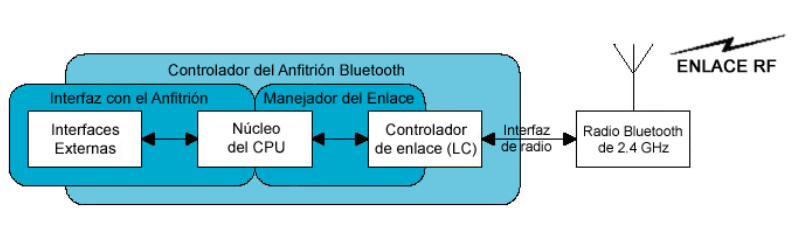
\includegraphics[width=15cm]{graphs/bluetooth_hardware.png}
	\caption{Arquitectura de Hardware del protocolo Bluetooth \cite{codificacion}}
	\label{figure:bluetoothhw} 
\end{figure}

El controlador digital esta compuesto por un CPU, por un procesador de señales digitales llamado Controlador de Enlace y por los interfaces con el dispositivo anfitrión. El controlador de enlace se encarga de hacer el procesamiento de la banda base y del manejo de los protocolos ARQ y FEC de la capa física para el manejo y corrección de errores. Además, se encarga de las funciones de transferencia (tanto asíncrona como síncrona), codificación de audio y encripción de datos. El CPU del dispositivo se encarga de atender las instrucciones relacionadas con Bluetooth del dispositivo anfitrión, para así simplificar su operación. Para ello, sobre el CPU corre un software denominado Manejador del Enlace, que tiene la función de comunicarse con otros dispositivos por medio del protocolo LMP.

\subsubsection{Arquitectura de Software}
Buscando ampliar la compatibilidad de los dispositivos Bluetooth, los dispositivos que se apegan al estándar utilizan como interfaz entre el dispositivo anfitrión (ordenador portátil, teléfono celular, etcétera) y el dispositivo Bluetooth como tal (chip Bluetooth) una interfaz denominada HCI (Host Controller Interface).

Los protocolos de alto nivel como el SDP (Protocolo utilizado para encontrar otros dispositivos Bluetooth dentro del rango de comunicación, encargado, también, de detectar la función de los dispositivos en rango), RFCOMM (Protocolo utilizado para emular conexiones de puerto serial) y TCS (Protocolo de control de telefonía) interactúan con el controlador de banda base a través del Protocolo L2CAP (Logical Link Control and Adaptation Protocol). El protocolo L2CAP se encarga de la segmentación y re-ensamblaje de los paquetes para poder enviar paquetes de mayor tamaño a través de la conexión Bluetooth. 

La arquitectura de software completa puede contemplarse en la figura \ref{figure:bluetoothsw}.

\begin{figure}[h] \centering
	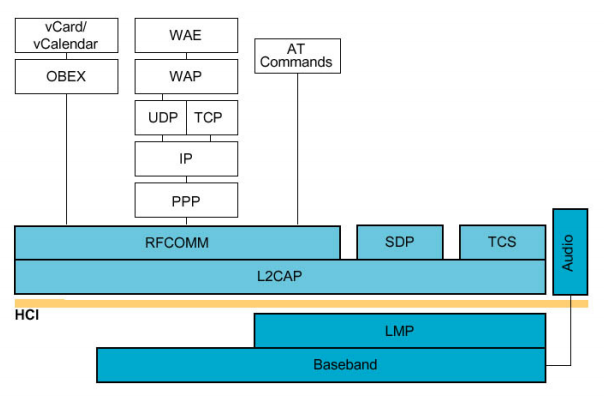
\includegraphics[width=15cm]{graphs/bluetooth_arquitectura_protocolos.png}
	\caption{Arquitectura de Software del protocolo Bluetooth \cite{codificacion}}
	\label{figure:bluetoothsw} 
\end{figure}

\subsection{Bluetooth de baja energía}

Bluetooth es uno de los protocolos inalámbricos más populares, y ha estado disponible en los teléfonos inteligentes, computadoras y otros dispositivos durante más de una década. El crecimiento explosivo de los dispositivos Bluetooth llevó a Bluetooth \ac{SIG} y a distintas empresas a la realización de que Bluetooth consumía demasiada energía y empleaba demasiado tiempo para conectarse en ciertas aplicaciones.

Bluetooth v4.0 introdujo \ac{BLE} , oficialmente conocido como \tit{Bluetooth Smart} o Bluetooth Inteligente. Esta especificación introduce un estándar radio completamente diferente, utilizando menos energía y con un coste menor, para así satisfacer las necesidades de estas nuevas aplicaciones. El amplio soporte de \ac{BLE} en teléfonos inteligentes y tabletas hace que las aplicaciones BLE sean fáciles de implementar y fáciles de usar para los consumidores.

El iPhone 4s de Apple introdujo soporte para \ac{BLE} y abrió el camino a un número masivo de dispositivos pequeños que son capaces de funcionar con pequeñas baterías. Antes de \ac{BLE}, el Bluetooth Clásico necesitaba baterías mas grandes por el gran uso de energía, y también requería de un chip de autentificación que era costoso. \ac{BLE} resuelve estos problemas para conectarse con iPhones y iPads. Muchos teléfonos basados en Android también presentan soporte para \ac{BLE}, concretamente desde la versión de Android 4.3. El \ac{SIG} de Bluetooth predice que para el 2018 más del 90 \% de los teléfonos móviles soportarán \ac{BLE}

Uno de los aspectos más poderosos de BLE es su flexibilidad y baja energía, que permite intercambiar información en forma genérica, a diferencia de la estructura rígida del Bluetooth Clásico.

\subsubsection{Comparación con otros protocolos}

Bluetooth y \ac{BLE} son protocolos que pueden simplificar la conectividad de productos, pero es importante entender como se comparan a otras tecnologías inalámbricas. WiFi, Zigbee y otros protocolos son mejores en ciertas aplicaciones  y \ac{BLE} no es siempre la mejor solución. La tabla \ref{table:blecomparison} muestra algunas de las características que diferencian a \ac{BLE} de ellos:

\begin{table}[H]%
	\centering
	\begin{tabular}{|c|c|c|c|}
		\hline
		\hline
		\tbf{}&\tbf{BLE} &\tbf{Wi-Fi}&\tbf{Zigbee}\\ \hline 
		\tbf{Banda de Frecuencia}&2.4 GHz&2.4 GHz / 5 GHz&2.4 GHz\\ \hline
		\tbf{Modulación}&GFSK&OFDM, DSSS&DSSS\\ \hline
		\tbf{Rango}&< 100m&< 300m&< 100m Punto a Punto\\ \hline
		\tbf{Topología de Red}&Scatternet&Star&Mesh\\ \hline
		\tbf{Velocidad}&1 Mbps&\specialcell{11 Mbps, 54 Mbps \\ 150 Mbps+}&250 kbps\\ \hline
		\tbf{Corriente Pico}&<15 mA&\specialcell{60 mA Rx \\ 200 mA Tx}&\specialcell{19mA Rx \\ 35mA Tx}\\ \hline
		\tbf{Corriente en Espera}&< 2 $\mu$A&< 100 $\mu$A&5 $\mu$A\\ \hline
		\hline 
	\end{tabular}
	\caption{Comparación de BLE con otros protocolos \cite{bluetoothlowenergy}}
	\label{table:blecomparison}
\end{table} 

Zigbee, Wi-Fi y \ac{BLE} utilizan la banda ISM de 2,4 GHz, pero son muy diferentes en sus capacidades. El transmisor \ac{BLE} es claramente un dispositivo de menor alcance que consume menos energía que Zigbee y especialmente Wi-Fi. El consumo de corriente pico más bajo es fundamental en el momento de elegir una batería. Wi-Fi, con un máximo de 200 mA nunca podría operar con una pila de botón. La corriente pico de \ac{BLE}, sin embargo, es mucho más baja.

A diferencia de Zigbee, \ac{BLE} no puede actualmente formar una red de malla, aunque si hay empresas que proveen de implementaciones específicas. Comunicación Punto a Punto implica que los dispositivos tienen que estar en el rango del teléfono inteligente para controlarlo. También hay soluciones utilizando una pasarela inalámbrica que conecta dispositivos \ac{BLE} a un enrutador, pero estos aumentan el coste final del producto.

\subsubsection{Capa física BLE}

\begin{figure}[h] \centering
	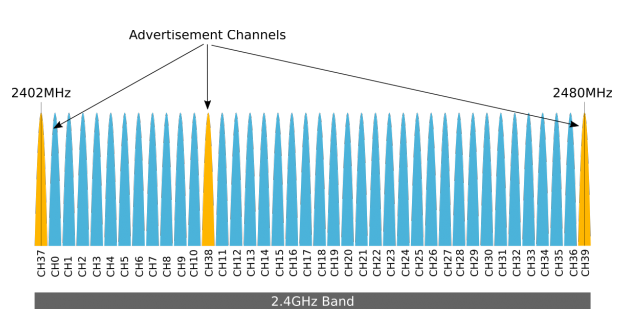
\includegraphics[width=15cm]{graphs/ble_capa_fisica.png} 
	\caption{Capa Física BLE \cite{bluetoothlowenergy}}
	\label{figure:capafisica}
\end{figure}

La capa física se relaciona directamente con la manera en la que los dispositivos \ac{BLE} transmiten y reciben datos.

\ac{BLE} utiliza la misma banda \ac{ISM} de 2,4 GHz que Bluetooth Clásico, abarcando desde 2400 MHz hasta 2483.5 MHz. Bluetooth v4.0 y especificaciones posteriores dividen la banda en 40 canales. Tal y como muestra la figura \ref{figure:capafisica}, 3 de estos canales son llamados “publicidad” y son utilizados por los dispositivos para enviar paquetes de publicidad con información sobre ellos para que otros dispositivos \ac{BLE} puedan conectarse. Estos canales se seleccionaron en la parte baja, media, y alta de la banda para evitar la interferencia de Wi-Fi. Por ejemplo, si el Canal 38 y canales cercanos están siendo interferidos por Wi-Fi, entonces todavía hay otros 2 canales de publicidad 37 y 39, que no se verán afectados y que \ac{BLE} puede usar.

\subsubsection{Capa de Enlace de Datos}
El verdadero funcionamiento de \ac{BLE} sucede en lo que se llama la capa de Enlace. Esta es la capa que tiene como funciones principales gestionar las conexiones y controlar los paquetes enviados y recibidos. Un dispositivo \ac{BLE} presenta varios estados posibles, aunque solo uno de ellos es permitido a la vez:

\begin{itemize}
\item Espera \\ El dispositivo no está transmitiendo o recibiendo, si no que está ``dormido'' para así ahorrar energía.
\item Publicidad \\ Un dispositivo que tiene un papel periférico entrará en el estado de publicidad, donde se enviarán paquetes en los canales de publicidad. En este estado también escuchará las respuestas a los paquetes desde un dispositivo central. Este modo es uno de los más críticos de entender desde una perspectiva de energía debido a que un dispositivo periférico pasará gran parte de su tiempo en el modo de Publicidad (dependiendo de la aplicación). El intervalo de Publicidad pues afecta directamente al consumo y duración de la batería.
\item Escaneo \\  Escaneo se refiere a escuchar los paquetes de publicidad que se envían a través de esos canales. Este modo se utiliza para buscar los dispositivos.
\item Iniciador \\ Este estado es el estado en el que un dispositivo central generalmente entra antes de establecer una conexión. El dispositivo central va a escuchar anuncios en los periféricos, pero una vez que el anuncio de la periférica deseada se recibe en el dispositivo, la central puede conectarse mediante el envío de los datos correctos.

Para el dispositivo esclavo, el estado Publicidad es también el estado inicial antes del estado de conexión. El estado de conexión es el estado final en el que el esclavo (periférico) y maestro (central) pueden intercambiar datos.
En \ac{BLE}, los datos se intercambian periódicamente sobre eventos de conexión.

Los datos se transmiten en los canales de datos, que son los 37 canales no utilizados para la publicidad. Ambos dispositivos se pondrán de acuerdo sobre los canales a usar y alternarán el envío de los datos, siguiendo las normas establecidas por la especificación.

Una aplicación típica \ac{BLE} implica un chip conectado a diversos sensores. Un usuario con un teléfono inteligente entra en el rango del dispositivo \ac{BLE}. El sensor con BLE transmite paquetes de publicidad y una vez que el teléfono recibe el anuncio del paquete, comenzará el proceso de conexión para obtener los datos de los sensores.

\end{itemize}

\FloatBarrier
\section{Android}
\label{sec:AndroidIntro}
    Android es un sistema operativo que en sus inicios fue concebido para dispositivos móviles con pantalla táctil. Sin embargo, ha evolucionado en una plataforma que actualmente también engloba relojes inteligentes, televisores, automóviles e incluso electrodomésticos.

\begin{figure}[h] \centering
    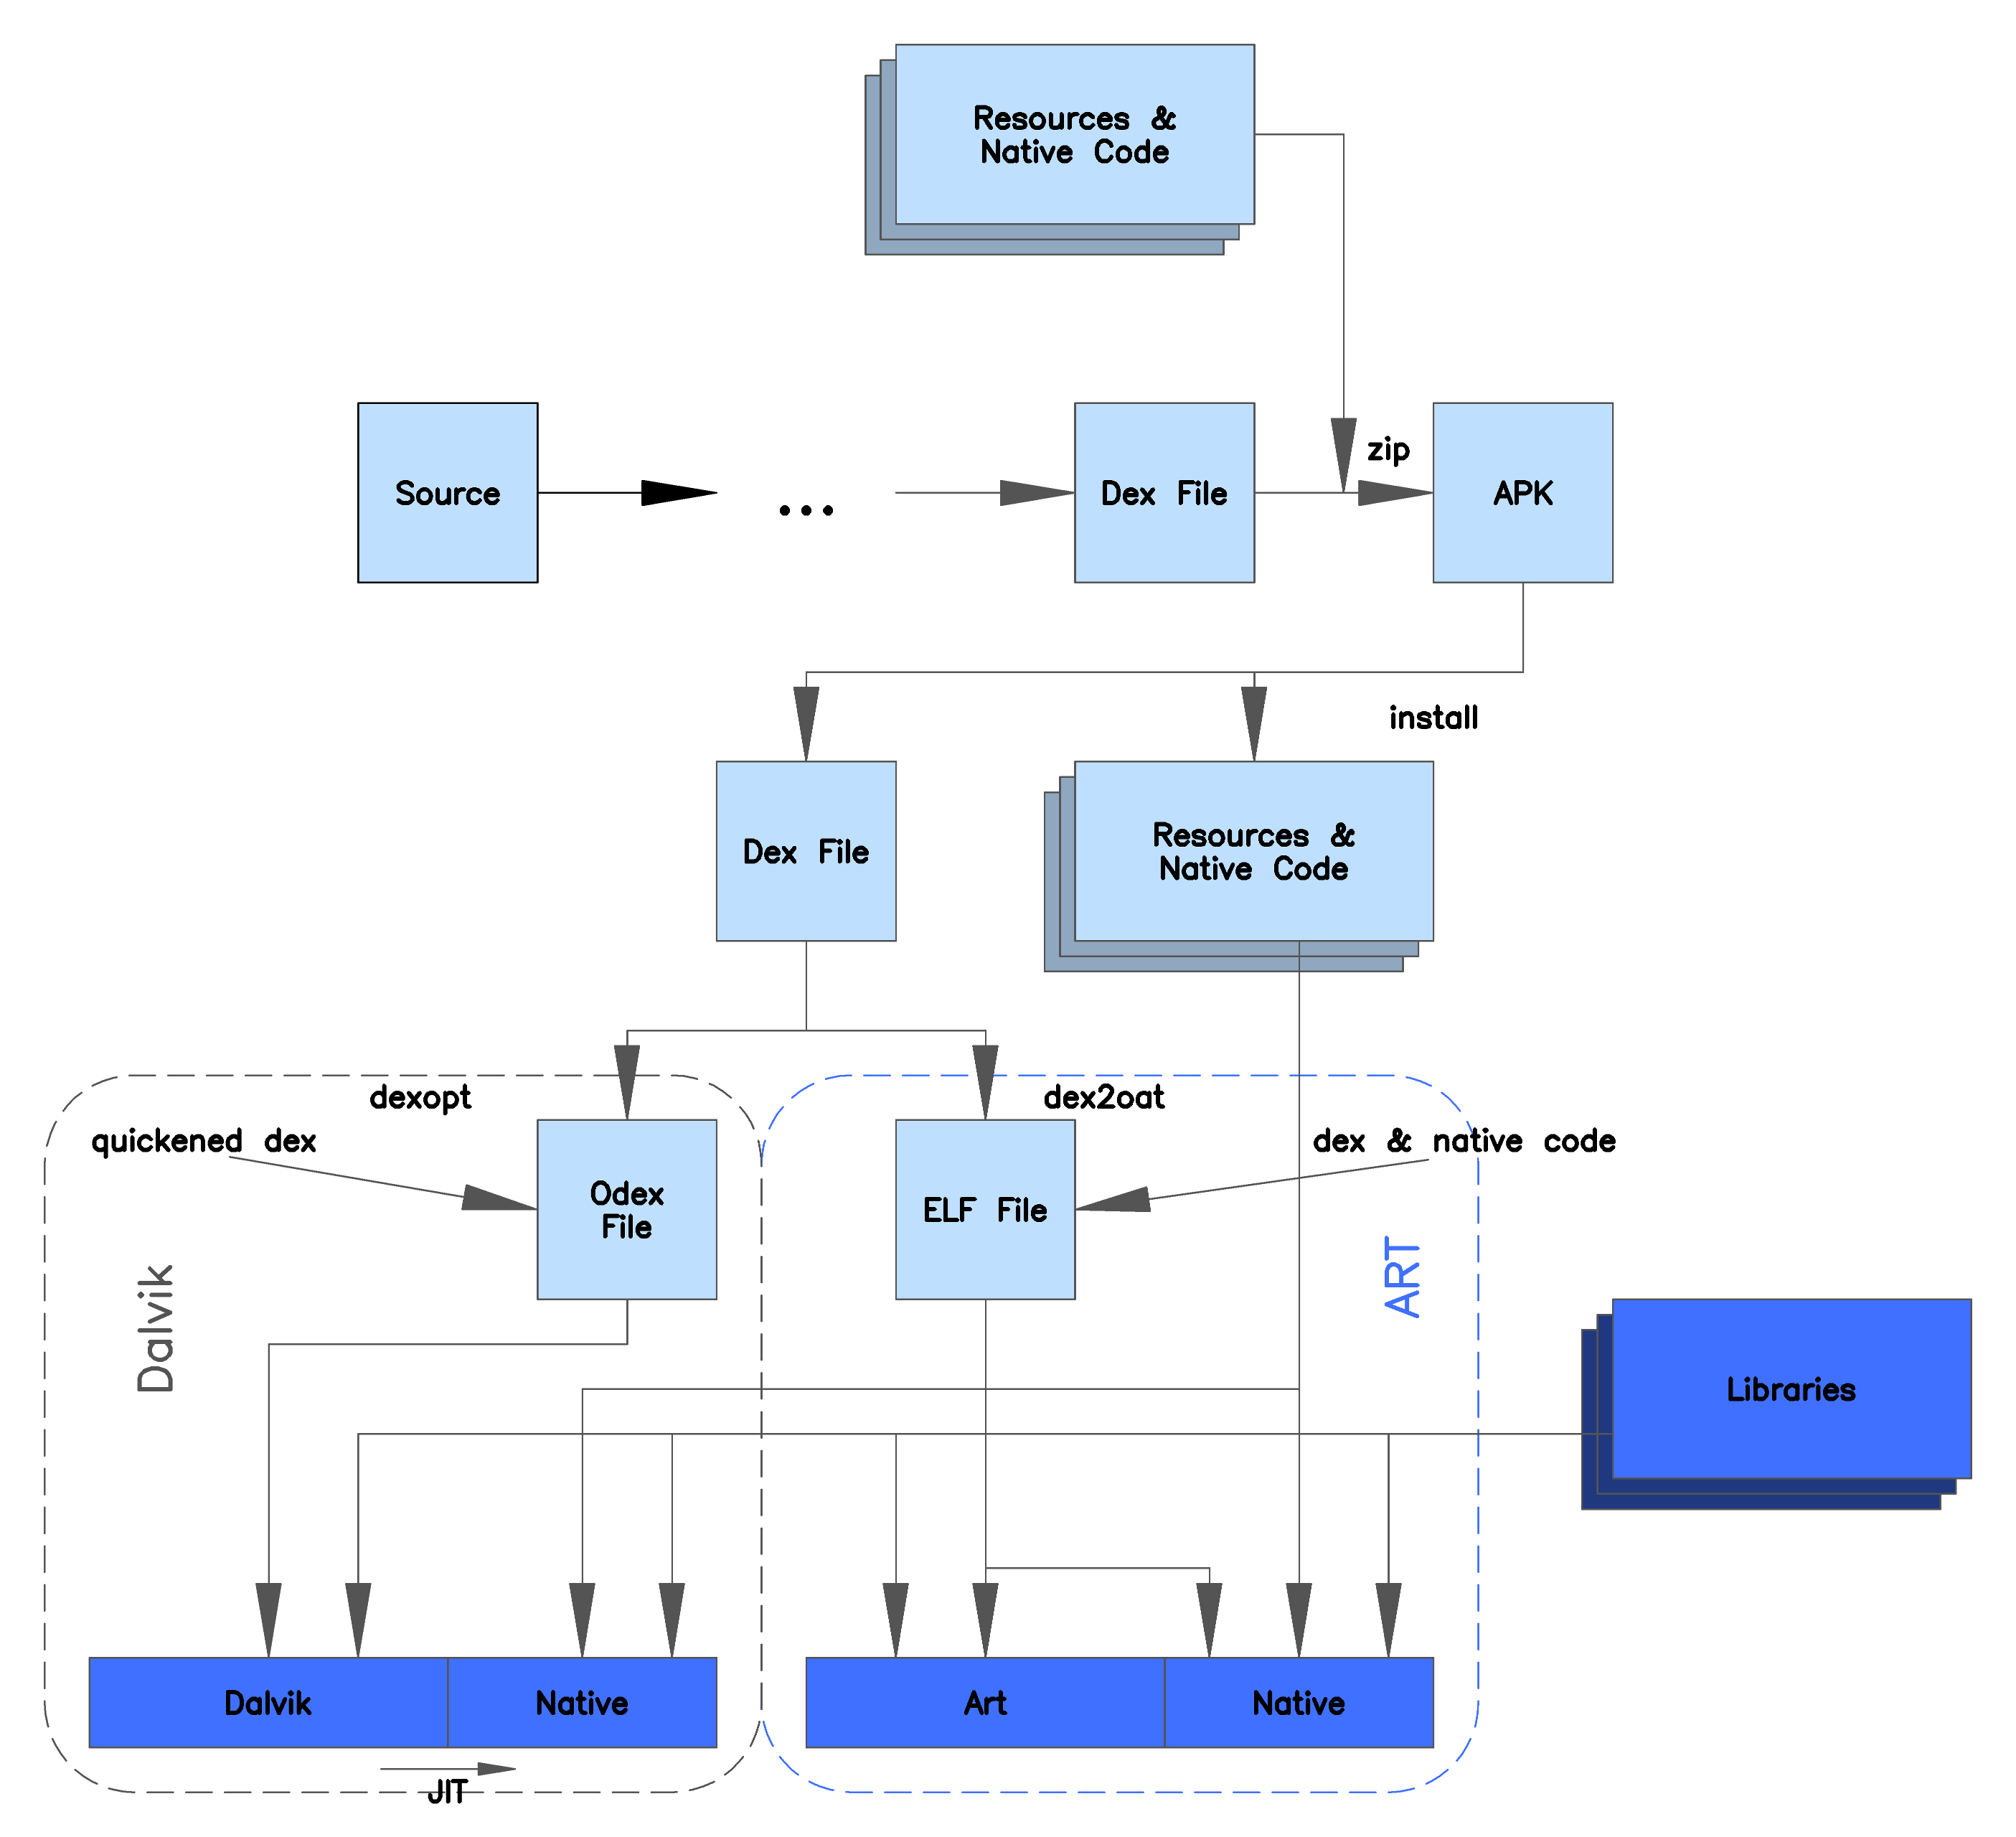
\includegraphics[height=12cm]{graphs/ART_view.png} \caption{Diagrama de la estructura del sistema operativo Android\cite{androiddevguide} }\label{fig:diagrama:ART}
\end{figure}

    Está basado en el núcleo de Linux. Sobre este, corre el entorno de ejecución propio de Android, que provee una máquina virtual (ya sea Dalvik o ART). Este a su vez ejecuta el código de las aplicaciones, escritas mayoritariamente en Java, aunque se permiten extensiones en C/C++. Las aplicaciones son precompiladas a un código intermedio denominado \ttw{Dex} y este es empaquetado y comprimido en el archivo estándar de aplicación Android, el \ttw{APK}. 

    Cada aplicación instalada en el dispositivo, es optimizada según los recursos y tipo de máquina virtual disponibles en el dispositivo en concreto. Al ser iniciada, es ejecutada dentro de un ``cajón de arena'', técnica que aísla los procesos de cada aplicación. Esto resulta en una mayor robustez y seguridad del sistema, ya que el fallo de una aplicación no afecta a los recursos de las demás. Tampoco podría una aplicación maligna, si se diera el caso, modificar o apropiarse de los recursos de otras. En la figura \ref{fig:diagrama:ART} se observa la relación entre todos los elementos anteriormente descritos.

\subsection{Interfaz}
    La interfaz de usuario por defecto de Android está basada en una manipulación directa, usando entrada táctil con gestos que vagamente corresponden a acciones físicas reales, tales como deslizar, golpear, pellizcar, etcétera. Para manipular objetos en pantalla. Además, la mayoría de dispositivos dispone de un teclado virtual, manipulado de la misma manera. 

    La respuesta del sistema a la entrada del usuario está diseñada para ser inmediata y dar una sensación de fluidez, utilizando las capacidades de vibración presentes en la mayoría de los dispositivos para proveer una respuesta háptica (no visual, no auditiva). Adicionalmente, algunas aplicaciones utilizan la información proveída por sensores tales como acelerómetros, giroscopios y sensores de proximidad para responder a interacciones adicionales, como por ejemplo ajustar la orientación de la pantalla cuando el dispositivo se encuentra apaisado o controlar alguna parte de la aplicación basándose en el azimut relativo del dispositivo.

\begin{figure}[h] \centering
    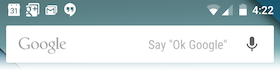
\includegraphics[width=8cm]{graphs/notification_area.png} \caption{Notificaciones minimizadas en el área de notificaciones\cite{androiddevguide} }\label{fig:screen:notification}
\end{figure}

    Una parte importante de la interfaz general de Android son las notificaciones, presentes en la barra de estado. Una notificación es un mensaje que una aplicación muestra al usuario fuera de los límites habituales de la interfaz de usuario de la aplicación. Las aplicaciones solicitan al sistema que emita una notificación por ellas, proveyendo el contenido, y el sistema operativo es quien maneja el resto del ciclo de vida de la notificación. En la figura \ref{fig:screen:notification} se pueden observar cuatro notificaciones minimizadas en el área de notificaciones

\subsection{Componentes de una aplicación}

\subsubsection{Contexto}
    Uno de los conceptos más importantes cuando se utiliza la plataforma Android es el contexto, \ttw{Context}. La clase \ttw{Context} en si misma no es más que una interfaz a información global acerca del entorno de una aplicación, y como tal es abstracta. Sin embargo, es importante ser consciente de qué elementos representan un contexto válido y qué elementos no. Un contexto permite acceso a recursos y clases específicos de la aplicación, y llamadas al sistema para operaciones a nivel de aplicación. Por ejemplo lanzar actividades, emitir mensajes de difusión o recibirlos.

\subsubsection{Actividades}
    En Android, una actividad (\ttw{Activity}) representa una única cosa concreta que el usuario puede realizar en la aplicación. La mayoría de las actividades interaccionan con el usuario, por tanto la clase \ttw{Activity} se encarga de crear una ventana donde se puedan insertar los componentes de la interfaz de usuario. Aunque las actividades suelen ser vistas por el usuario como ventanas a pantalla completa, también pueden ser usadas en otras múltiples maneras, ya sea como ventanas flotantes, o incrustadas dentro de otra actividad (mediante un \ttw{ActivityGroup})

\subsubsection{Ciclo de vida de una actividad}
    Las distintas actividades de las distintas aplicaciones instaladas en el dispositivo Android son gestionadas en forma de una ``pila de actividades''.
 
    Cuando el sistema Android se inicia, se presenta al usuario una pantalla principal, desde donde puede lanzar varias acciones y aplicaciones. A partir de ahí, cuando una nueva actividad es empezada, se emplaza arriba de la pila y se convierte en la actividad en ejecución. Las actividades previas, si las hubiera, siempre permanecen por debajo en la pila, y no se traerán al frente hasta que la nueva actividad finalice.

\begin{figure}[!htbp] \centering
    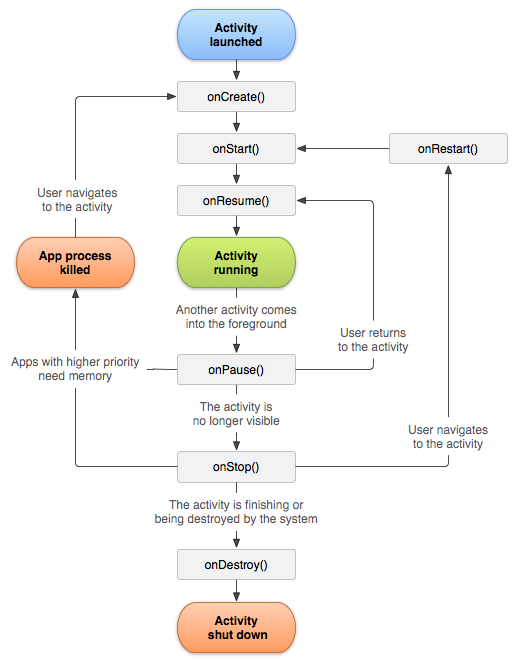
\includegraphics[width=12cm]{graphs/activity_lifecycle.png} \caption{Diagrama del ciclo de vida de una actividad en Android \cite{androiddevguide}.}\label{fig:diagrama:ActivityLifecycle}
\end{figure}

Una actividad tiene cuatro estados básicos:

\begin{description}
    \item[Activa] \hfill \\
     Una actividad está \tit{activa} cuando está presente en primer plano en la pantalla, es decir, arriba de la pila. También se puede decir que la actividad está \tit{En ejecución}.

    \item[Pausada] \hfill \\
    Si una actividad ha perdido el foco (ha dejado de estar en primer plano) pero todavía es visible, es decir, si una nueva actividad que no ocupa la totalidad de la pantalla o es transparente obtiene el primer plano, se encuentra \tit{pausada}. Una actividad pausada se conserva completamente íntegra (mantiene todos los estados y se mantiene suscrita al gestor de ventanas) pero puede ser matada por el sistema en condiciones extremas de baja memoria disponible.

    \item[Parada] \hfill \\
    Si una actividad se encuentra oculta por completo, el sistema la deja \tit{parada}. Mantiene estados e información de los miembros, pero sin embargo al no ser visible por el usuario es más probable que el sistema se deshaga de ella para liberar recursos cuando hagan falta.
    
    \item[Muerta] \hfill \\
    Cuando el sistema decide mover la actividad fuera de memoria, puede o bien finalizarla o matar el proceso. Cuando sea mostrada de nuevo al usuario, debe ser completamente reiniciada y restaurada a su estado previo.
\end{description}

    Los cuatro estados y las acciones que llevan a una aplicación de un estado a otro, junto con los métodos de la actividad que son invocados en cada etapa, están representados en la figura \ref{fig:diagrama:ActivityLifecycle}.

\FloatBarrier
\subsubsection{Servicios}
\label{ssec:teo:svc}

Un Servicio (\ttw{Service}) es un componente de la aplicación que puede realizar tareas de larga duración en segundo plano y no provee ninguna interfaz de usuario. Otro componente de la aplicación puede iniciar un servicio y este continuará en marcha en segundo plano, incluso si el usuario cambia a otra aplicación distinta. Además, un componente puede adherirse (\ttw{bind}) a un servicio para interactuar con él, e incluso realizar comunicación inter-procesos (IPC por sus siglas en inglés, Inter-Process Communication). Por ejemplo, un servicio puede manejar llamadas de red, reproducir música, realizar operaciones en el sistema de archivos, todo en segundo plano.

Un servicio puede tomar dos estados:

\begin{description}
    \item[Started] \hfill \\
    Un servicio está en estado \ttw{Started} (empezado) cuando un componente de la aplicación, por ejemplo una actividad, lo empieza llamando al método \ttw{startService()}. Una vez empezado de esta manera, un servicio puede continuar en segundo plano de manera indefinida, incluso si el componente que lo empezó ha sido destruido. Normalmente, suelen ser servicios que realizan una única operación y no devuelven ningún resultado. Por ejemplo, puede descargar o subir un archivo en la red. Cuando la operación ha sido completada, el servicio debe pararse a si mismo.
    
    \item[Bound] \hfill \\
    Un servicio está en estado \ttw{Bound} (adherido) cuando un componente de la aplicación se adhiere a él llamando al método \ttw{bindService()}. Un servicio adherido ofrece una interfaz servidor-cliente que permite a los componentes interaccionar con el servicio, mandar peticiones, obtener resultados, e incluso hacerlo entre distintos procesos mediante comunicación inter-proceso (IPC). Un servicio adherido solamente es activo durante el tiempo que otro componente esté adherido a él. Varios componentes pueden estar adheridos en un momento dado al servicio, pero cuando todos se desadhieren del servicio, el servicio es destruido.

\end{description}

\begin{figure}[h] \centering
    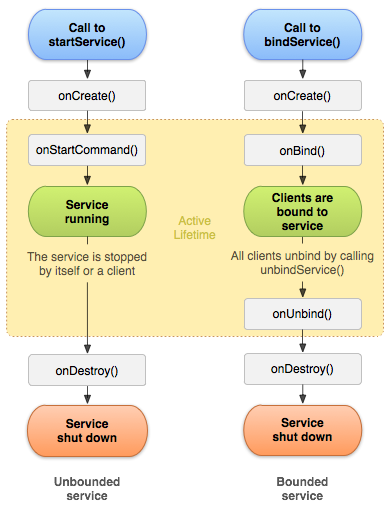
\includegraphics[width=9cm]{graphs/service_lifecycle.png} \caption{Diagrama del ciclo de vida de un servicio \cite{androiddevguide}}.\label{fig:diagrama:ServiceLifecycle}
\end{figure}

    Es necesario tener cuidado, dado que un servicio corre en el hilo principal de ejecución del proceso que lo llama, a no ser que se especifique lo contrario. Esto implica que, si el servicio va a realizar alguna tarea intensiva en CPU, o alguna operación bloqueadora, se debe de crear un nuevo hilo de ejecución dentro del servicio para ese propósito. De no hacerlo, se corre el riesgo de que la aplicación deje de responder y sea matada por el sistema operativo.

    Los dos tipos de ciclo de vida de un servicio, sus etapas y los métodos invocados en el transcurso de ellas están representados en la figura \ref{fig:diagrama:ServiceLifecycle}.

\FloatBarrier
\subsection{Vistas}
La interfaz gráfica de usuario en una aplicación Android está construida usando una jerarquía de vistas, objetos de la clase \ttw{View}, y grupos de vistas, objetos de la clase \ttw{ViewGroup}. Los objetos \ttw{View} suelen ser artilugios (widgets) de la interfaz de usuario, tales como botones o campos de texto, y los objetos \ttw{ViewGroup} son contenedores invisibles que definen cómo se posicionan las vistas que dependen de ellos, por ejemplo dispuestas en forma de rejilla o lista vertical.

Android provee un vocabulario XML que se corresponde con las subclases de \ttw{View} y \ttw{ViewGroup}, y permite definir la interfaz de usuario en XML usando una jerarquía de elementos de interfaz de usuario.

\subsection{Procesos e hilos de ejecución}
    En sistemas operativos, son básicos los conceptos de proceso e hilo de ejecución. En Android, el sistema operativo comienza un nuevo proceso Linux por cada primer componente de cada aplicación, con un único hilo de ejecución. Por defecto, todos los componentes de la misma aplicación corren en los mismos proceso e hilo de ejecución, el hilo principal de ejecución (\tit{main thread} en inglés). 

    En caso de que un componente de una aplicación sea inicializado, y ya exista un proceso para dicha aplicación en el sistema que otro componente de la misma aplicación ha inicializado, el nuevo componente se inicializa dentro del proceso original y usa el mismo hilo de ejecución. Sin embargo, se puede configurar una aplicación de manera que diferentes componentes corran en procesos separados, y siempre se pueden crear hilos de ejecución adicionales para cualquier proceso.

\subsubsection{Procesos}
    Como ya ha sido expuesto anteriormente, por defecto todos los componentes de la misma aplicación corren en el mismo proceso, y la mayoría de las aplicaciones no deberían de cambiarlo. Sin embargo, es posible controlar qué proceso pertenece a qué componente de ser necesario.

    El sistema operativo puede decidir apagar un proceso, cuando la cantidad de memoria disponible sea baja y haya requerimiento de ella por otro proceso que sirva de manera más inmediata al usuario. En este caso, los componentes dentro de dicho proceso que es apagado, son destruidos. Cuando estos componentes sean necesarios de nuevo, un nuevo proceso será comenzado por el sistema operativo para ello.

\subsubsection{Hilos de ejecución}
    Previamente se ha mencionado que todos los componentes de la misma aplicación corren en el mismo hilo de ejecución, el hilo principal de ejecución o \tit{main thread}. Este hilo es de suma importancia, dado que carga con la responsabilidad de despachar los eventos al widget de la interfaz de usuario que sea pertinente, incluyendo los eventos de dibujado en pantalla. Es también el hilo de ejecución en el que la aplicación interactúa con los componentes básicos de interfaz de usuario de Android, también conocidos como \tit{Android UI toolkit} (ubicados dentro de los paquetes java \ttw{android.widget} y \ttw{android.view}). Por todo esto, no es extraño encontrar denominado este hilo de ejecución como el hilo de la interfaz de usuario, o \tit{UI Thread}.

    Dado que todos los componentes que corren en el mismo proceso son instanciados en el hilo de ejecución principal, las llamadas del sistema operativo a cada componente son despachadas desde dicho hilo. En consecuencia, todos los métodos que responden a retrollamadas del sistema (\tit{system callbacks}), como por ejemplo para indicar que una tecla ha sido pulsada, siempre corren en el hilo principal de ejecución del proceso.

    Cuando el usuario toca un botón en la pantalla, el hilo principal de la aplicación despacha el evento de toque al widget pertinente, que reacciona cambiando su estado a presionado y manda una petición de invalidación a la cola de eventos. El hilo de ejecución principal entonces desencola la petición y notifica al widget que debe de re-dibujarse.

    Cuando una aplicación realiza trabajo intensivo en respuesta a una interacción del usuario, el modelo de hilo de ejecución único puede resultar en una falta de rendimiento. Concretamente, de suceder todo el procesamiento en el hilo principal de ejecución e iniciar tareas de larga ejecución tales como acceso a red o consultas a bases de datos, resultará en un bloqueo completo de la interfaz de usuario y su correspondiente hilo principal. Cuando el hilo de ejecución está bloqueado, no se pueden despachar eventos, eventos de dibujado en pantalla incluidos. Desde el punto de vista del usuario, esto se traduce en una aplicación que parece colgarse. En peores casos, en los que el hilo principal de ejecución está bloqueado por más de unos cuantos segundos (cinco segundos en la actualidad) el sistema operativo entrará en acción y mostrará una pantalla explicando que la aplicación ha dejado de responder, y matará la aplicación bloqueada. 

    Para evitar dicha penalización en el rendimiento, deben usarse hilos de ejecución alternativos para toda tarea que bloquee la ejecución o sea de alta carga procedural.

\FloatBarrier

\subsection{Ubicación}
\subsubsection{GPS}
El \ac{GPS} es un sistema de navegación por satélite que provee información sobre la posición y el reloj del dispositivo de recepción. El sistema fue desarrollado, instalado y empleado por el Departamento de Defensa de los Estados Unidos. Está constituido por 24 satélites en órbita geosíncrona y se basa en un sistema de triangulación para determinar posiciones con precisión de metros.

El funcionamiento del \ac{GPS} necesita la recepción de la señal de al menos cuatro de los 24 satélites en órbita. En base a dichas señales, que incluyen la identificación del satélite emisor y la hora de reloj de emisión, el aparato receptor sincroniza su reloj interno y calcula el tiempo que tardan en llegar las señales al equipo. Con dicha información, el dispositivo es capaz de conocer su distancia a cada uno de los satélites cuya señal es recibida, y por ende la posición absoluta del punto de medición.

\subsubsection{Servicios Móviles de Google}
Conocer la localización \ac{GPS} del dispositivo móvil es crítico en el funcionamiento de la aplicación. Es posible en un dispositivo Android utilizar el receptor \ac{GPS} a bajo nivel y recibir actualizaciones de posición en formato NMEA. Sin embargo, no se aprovecharían cantidad sustancial de optimizaciones que Google ofrece como parte de \ac{GMS} tales como tiempo de respuesta mejorado, localización mixta y consumo de batería mejorado. 

\ac{GMS} es un servicio en segundo plano propietario de Google presente en todos los dispositivos Android que satisfagan las condiciones de entrada de la empresa. En este proyecto, la aplicación se conectará a dicho servicio para requerir actualizaciones de posición.

\subsection{BLE en Android}
 Android 4.3 (Nivel API 18) introduce una función de soporte de la plataforma para Bluetooth de baja energía y proporciona una API que las aplicaciones pueden utilizar para detectar dispositivos \ac{BLE}, consultar servicios y realizar operaciones de lectura o escritura. En contraste con el Bluetooth clásico, \ac{BLE} está diseñado para proporcionar un consumo de energía significativamente menor. Esto permite que aplicaciones Android puedan comunicarse con dispositivos BLE que tienen requisitos de baja potencia, tales como sensores de proximidad, pulsómetros, sensores publicitarios y otros muchos más.
 
\subsubsection{Conceptos y Terminología clave}
A continuación presentamos un resumen de los conceptos y terminología que son de vital importancia cuando hablamos del protocolo BLE:
\begin{itemize}
\item \ac{GATT} \\ El \ac{GATT} es una especificación general para el envío y recepción de pequeñas cantidades de datos conocidos como ``atributos'' a través de un enlace BLE. Todos los perfiles actuales de aplicaciones de baja energía se basan en el GATT.
El SIG de Bluetooth define muchos perfiles para dispositivos de baja energía. Un perfil es una especificación para el funcionamiento de un dispositivo en una aplicación particular, teniendo en cuenta que un dispositivo puede aplicar más de un perfil. Por ejemplo, un dispositivo podría contener un monitor de ritmo cardíaco y un detector de nivel de batería.
\item \ac{ATT} \\ \ac{GATT} se define encima del protocolo \ac{ATT}. El conjunto también se conoce como el protocolo GATT/ATT. ATT está optimizado para funcionar en dispositivos BLE. Con este fin, se utiliza el menor número de bytes posible. Cada atributo está identificado por un identificador único universal (UUID), que es una cadena de caracteres representando un identificador con un formato de 128 bits normalizado, para así identificar de forma unívoca la información. Los atributos transportados por ATT reciben el nombre de características y servicios.
\item Característica \\ Una característica contiene un único valor y 0-n descriptores que describen el valor de dicha característica. Una característica puede ser interpretada como un tipo, análogo a una clase en \ac{POO}
\item Descriptor \\ Los descriptores son atributos definidos que describen el valor de una característica. Por ejemplo, un descriptor podría especificar una descripción legible por el ser humano, un rango aceptado para el valor de una característica, o una unidad de medida que es específica a un valor de una característica determinada.
\item Servicio \\ Un servicio es una colección de características. Por ejemplo, un usuario podría disponer de un servicio llamado \tit{Monitor de Frecuencia Cardíaca}, el cual incluye características tales como \tit{Medida del ritmo cardíaco} o \tit{Posición del dispositivo medidor en el cuerpo humano}, entre otras.
\end{itemize}

\subsubsection{Roles y Responsabilidades}
Los roles y responsabilidades aplicables cuando un dispositivo Android interactúa con un dispositivo BLE son los siguientes:
\begin{itemize}
\item Central vs. periférica. Esto se aplica a la propia conexión BLE. El dispositivo con el rol o papel central escanea, en busca de publicidad, y el dispositivo con el rol periférico realiza el anuncio.
\item Servidor GATT vs. cliente GATT. Esto determina cómo se realiza la comunicación entre los dos dispositivos una vez que la conexión ha sido establecida.
\end{itemize}

\begin{figure}[h] \centering
 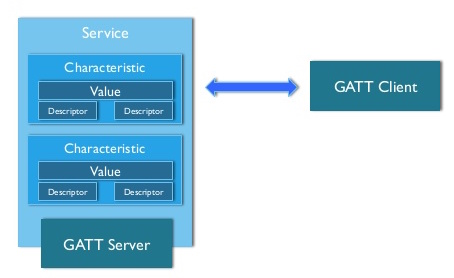
\includegraphics[height=7.5cm,keepaspectratio]{graphs/gattServerClient.png} \caption{Esquema Servidor y Cliente GATT \cite{androiddevguide}}\label{fig:gattconexion}
\end{figure}

Para entender la distinción, podemos imaginar que tenemos por un lado un teléfono Android y un rastreador de actividad como dispositivo BLE por otro. El teléfono es compatible con el papel central mientras que el rastreador de actividad se apoya en el papel periférico (para establecer una conexión BLE se necesitan dos dispositivos que presenten roles opuestos, ya que dos dispositivos que solo soporten modo periférico no podrían comunicarse entre sí, al igual que dos dispositivos que solo soportasen modo central).

Una vez que el teléfono y el rastreador de actividad han establecido una conexión, comienzan a transferir meta-datos GATT entre sí. Dependiendo del tipo de datos que se transfieren, el uno o el otro puede actuar como servidor. Por ejemplo, si el rastreador de actividad quiere reportar datos del sensor al teléfono, tendría sentido que el rastreador de actividad actuase como servidor. Si el rastreador de actividad quiere recibir actualizaciones desde el teléfono, entonces sería más conveniente designar al teléfono como el servidor, actuando el rastreador como cliente.

En nuestro caso particular, la aplicación Android (que se ejecuta en un dispositivo Android) es el cliente GATT. La aplicación recibe datos desde el servidor GATT, que es un pulsómetro comercial, el cual soporta el perfil BLE de ritmo cardíaco. La figura \ref{fig:gattconexion} muestra dicho esquema cliente-servidor.

\section{Desarrollo de aplicaciones web modernas}

\subsection{Definiciones básicas}

\subsubsection{Frontend}
El Frontend es un término muy utilizado en el desarrollo web actual, y podríamos resumirlo a que se refiere a la parte que el usuario común ve, es decir, la interfaz gráfica, aunque no se queda solo en eso, sino que dentro del Frontend podríamos decir que está el Javascript que se ejecuta del lado del cliente. Los lenguajes y tecnologías que componen el frontend son:

\begin{itemize}
\item \ac{HTML} \\ Define el contenido de una página web, como texto, imágenes y videos entre otros. Es un estándar a cargo de la W3C, organización dedicada a la estandarización de casi todas las tecnologías ligadas a la web, sobre todo en lo referente a su escritura e interpretación.
\item \ac{CSS} \\ Es un lenguaje usado para definir y crear la presentación de un documento estructurado escrito en HTML. La idea que se encuentra detrás del desarrollo de CSS es separar la estructura de un documento de su presentación.
\item Javascript \\ Es un lenguaje de programación interpretado, dialecto del estándar ECMAScript. Se define como orientado a objetos, basado en prototipos, imperativo, débilmente tipado y dinámico. En este caso nos referimos a Javascript del lado del cliente, implementado como parte de un navegador web, permitiendo mejoras en la interfaz de usuario y páginas web dinámicas.
\end{itemize}

\subsubsection{Backend}
Es lo que se ejecuta del lado del servidor. Los elementos del backend son los siguientes:

\begin{itemize}
\item Lógica de negocio.
\item Lenguaje de servidor (PHP, Ruby, Python, Javascript).
\item Bases de Datos
\end{itemize}

\subsubsection{Stack}
Un Stack, podríamos decir que es un conjunto de paquetes configurado de cierta manera que se complementan entre sí.
El ejemplo de un stack bastante conocido es LAMP, que es el conjunto de Linux, Apache, MySQL y PHP ejecutándose juntos como una plataforma para desarrollo web, o MEAN, el cual es bastante reciente y el usado en este proyecto, agrupando las tecnologías MongoDB, Express, AngularJS y Node.

\subsubsection{DOM}
\ac{DOM} es la estructura de objetos interna que genera el navegador cuando se carga un documento HTML y la cual se puede alterar mediante Javascript para cambiar de forma dinámica los contenidos y aspecto de la página. Es una estructura jerárquica donde existen varios objetos y unos dependen de otros.

Los objetos del DOM modelan tanto la ventana del navegador como el historial, el documento o página web, y todos los elementos que pueda tener dentro la propia página, como párrafos, divisiones, tablas, formularios y sus campos, etcétera. A través del DOM se puede acceder, por medio de Javascript, a cualquiera de estos elementos, es decir, a sus correspondientes objetos para alterar sus propiedades o invocar a sus métodos. Con todo, a través del DOM, queda disponible para los programadores de Javascript cualquier elemento de la página, para modificarlos, suprimirlos, crear nuevos elementos y colocarlos en la página, etcétera.

\subsubsection{Web Socket}
Especificación web que permite establecer una conexión persistente entre el cliente y el servidor, autorizando a ambas partes a enviar datos en cualquier momento.

\subsection{MEAN}
MEAN es un \tit{stack} para el desarrollo de aplicaciones web, el cual usa JavaScript como lenguaje de programación tanto para el frontend como para el backend, gracias a sus herramientas MongoDB, Express, AngularJS y NodeJS. Este es el motivo por el cual se denomina un \tit{full stack}. 
Podríamos considerarlo una alternativa a LAMP, aunque de cierta manera un poco lejana, ya que en LAMP utilizamos tecnologías distintas en cada cosa que queremos hacer.

\begin{table}[H]%
	\centering
	\begin{tabular}{|c|c|c|}
		\hline
		\hline
		\tbf{}&\tbf{LAMP/XAMPP} &\tbf{MEAN}\\ \hline 
		\tbf{Sistema Operativo}&\specialcell{Linux, Windows, \\ Mac OS X, etc...}&\specialcell{Linux, Windows, \\ Mac OS X, etc...}\\ \hline
		\tbf{Servidor HTTP}&Apache&Node.js\\ \hline
		\tbf{Base de Datos}&MySQL&MongoDB\\ \hline
		\tbf{Web Framework}&PHP&Express\\ \hline
		\tbf{Frontend Framework}&-&AngularJS\\ \hline
		\hline 
	\end{tabular}
	\caption{Comparación básica de LAMP y MEAN \cite{penflip}}
	\label{table:lampMean}
\end{table} 

\begin{table}[H]%
	\centering
	\begin{tabular}{|c|c|c|}
		\hline
		\hline
		\tbf{}&\tbf{LAMP} &\tbf{MEAN}\\ \hline 
		\tbf{Base}&Bash&Javascript\\ \hline
		\tbf{Servidor HTTP}&Apache Config&Javascript\\ \hline
		\tbf{Base de Datos}&SQL&Javascript\\ \hline
		\tbf{Lenguaje de Programación}&PHP&Javascript\\ \hline
		\hline 
	\end{tabular}
	\caption{Comparación entre lenguajes utilizados en LAMP y MEAN \cite{penflip}}
		\label{table:lampMeanLang}
\end{table} 

Como se puede observar en las tablas \ref{table:lampMean} y \ref{table:lampMeanLang} , lo único que comparten ambas pilas de desarrollo es la finalidad para la que se utilizan: desarrollo web. Otro de los puntos a revisar es el hecho de que LAMP no cuenta en sí con una librería JavaScript para el frontend, aunque podría usarse cualquier librería sin problema, como por ejemplo AngularJS o jQuery.

Por tanto, podemos decir que MEAN es un \tit{full stack} de desarrollo web con el que se pretende trabajar todo el tiempo con JavaScript. Este hecho se apoya en el gran progreso de optimización del lenguaje, llegando incluso a ser más rápido que otros lenguajes utilizados del lado del servidor, como PHP, Ruby y Python. 

A continuación vamos a analizar en detalle cada una de las herramientas y tecnologías que conforman el stack MEAN.

\subsection{MongoDB}
Sin duda alguna, MySQL es la base de datos más popular del mercado, aunque recientemente ha experimentado un bajón en su uso en favor de otros sistemas de gestión de bases de datos más abiertos, como MariaDB o PostgreSQL. Lo que tienen en común estos sistemas, es que son considerados ``Sistemas de Bases de Datos Relacionales'' y cumplen muy bien con su cometido, que es guardar información y recuperarla en cualquier momento con un alta disponibilidad. También tienen en común que para comunicarse con ellas necesitaremos dominar el lenguaje SQL.

El problema que presentan estas bases de datos son la velocidad de lectura cuando se tiene una gran demanda de datos y un crecimiento exponencial de la carga. Un ejemplo sencillo es el reflejado por las redes sociales, las cuales reciben miles de consultas por segundo que deben ser servidas de forma eficiente y siempre cuidando que, si hay algún error en uno de sus servidores, dicha información se encuentre disponible. 

Esta es una de las principales razones del nacimiento de las bases de datos NoSQL, que tal y como su nombre indica, no son bases de datos que se manejen con SQL y proveen una alta disponibilidad y eficiencia. Algunos ejemplos de estas bases de datos son MongoDB, HyperTable, Cassandra, CouchDB, etcétera.

Sin embargo, a pesar de que existen muchas alternativas de bases de datos NoSQL, podemos decir que pocas tienen la madurez, seguridad y velocidad necesarias para entrar en entornos de producción de alta exigencia. MongoDB es una de las pocas que puede hacer gala de ello, ya que presenta funciones bastante interesantes que la llevan a ser la base de datos favorita para muchas personas. A continuación destacamos los puntos clave:

\begin{itemize}
\item Desarrollada en C++ \\ C++ es un lenguaje de bajo nivel, lo que promete que alcanzará un gran rendimiento a la hora de exigirle. Los documentos son almacenados en estilo \ac{JSON}, por lo que no existen tablas, ni filas, ni columnas. Permite el uso de JavaScript para su manipulación.
\item Replicación \\ La base de datos incluye por defecto un sistema de replicación. Si introducimos un nuevo documento en nuestra base de datos, esta automáticamente lo replicará en otra base de datos en un servidor distinto. De esta manera nos aseguramos que nuestra información permanece segura y siempre disponible.
\item GridFS \\ Nos permite guardar documentos de cualquier tamaño sin afectar al rendimiento de la base de datos.
\end{itemize}

\subsection{Express}
Express es un framework de desarrollo de aplicaciones web minimalista y flexible para Node. Si bien la base sobre la que estaremos trabajando será Node, el sistema que nos ofrece por defecto para servir páginas es un poco complejo. Express nos abstrae de estas capas de bajo nivel, permitiéndonos crear un servidor web en muy pocos pasos.

Compite con rivales bastante fuertes en el mercado, como Meteor o Restify. Sin embargo, ninguno de ellos tiene la comunidad que Express tiene detrás brindando soporte. Prácticamente cualquier duda técnica que surja, podemos encontrar la solución en foros dedicados al soporte informático como StackOverflow o Quora. En cambio, otros frameworks, a pesar de ser muy buenos, no cuentan con esta ventaja.

Algunas de las características que Express nos ofrece son las siguientes:

\begin{itemize}
\item Sencillez
\item Comunidad bastante activa
\item Documentación de alta calidad
\item Compatibilidad con otros módulos
\item Alto Rendimiento, focalizándose en el enrutamiento
\end{itemize}

\subsection{AngularJS}
\label{angularJS}
AngularJS es un framework de JavaScript de código abierto, mantenido por Google, que ayuda con la gestión de lo que se conoce como aplicaciones de una sola página. Su objetivo es aumentar las aplicaciones basadas en navegador con capacidad de Modelo Vista Controlador (MVC), en un esfuerzo para hacer que el desarrollo y las pruebas sean más fáciles.

Algunas características que vienen acompañadas con AngularJS son:

\begin{itemize}
\item Comunidad \\ Al igual que Express, la comunidad es uno de sus puntos fuertes.
\item Herramientas \\  AngularJS proporciona numerosas herramientas que nos brindan facilidades con llamadas \ac{AJAX}, bucles, sistemas para clonado de objetos o arrays, sistema de monitorización de variables, etcétera.
\item Data-Binding \\ Se refiere a que, si desde el backend cambia de alguna manera el valor de una variable (y lo actualizamos en nuestro controlador), cambiará también en el frontend. Si en el frontend hay algún cambio, el valor de la variable automáticamente se actualizará sin tener que hacer llamadas extras para detectar dicho cambio. 
\item MVC \\ La forma en la que está estructurado AngularJS prácticamente nos obliga a tener nuestro código ordenado, utilizando controladores para mandar datos a la vista, además de modelos, directivas, servicios y filtros, entre otros.
\item Manejador de rutas \\ AngularJS incluye por defecto un manejador de rutas para implementar aplicaciones de una sola página, \tit{single page web applications}, es decir, compactar en una sola página todo el HTML y manejar toda la información mediante rutas y controladores, únicamente cargando lo que nos interesa y no toda la página. Con esto utilizamos menos recursos del servidor  y mejoramos el rendimiento desde el punto de vista del cliente con menos tiempo de carga y mejores respuestas.
\end{itemize}

Aunque profundizaremos a nivel técnico más adelante en el apartado \ref{Cliente}, se ha incluido en la figura \ref{ejemploAngular} un ejemplo sencillo de la sintaxis utilizada en AngularJS. Esta puede parecer un poco extraña al principio, pero que una vez que uno se acostumbra, es muy intuitiva y fácil de manejar.

\begin{figure}[h] \centering
	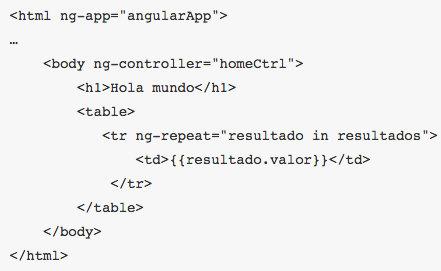
\includegraphics[height=7.5cm]{graphs/angular_example.png} \caption{Ejemplo de directivas AngularJS incrustadas en HTML \cite{penflip}}
	\label{ejemploAngular}
\end{figure}

\subsection{Node.js}
Node es un intérprete Javascript del lado del servidor que cambia la noción de cómo debería trabajar un servidor. Su meta es permitir a un programador construir aplicaciones altamente escalables y escribir código que maneje decenas de miles de conexiones simultáneas en una sola máquina física.

\subsubsection{¿Qué problema resuelve Node?}
La meta número uno declarada de Node es proporcionar una manera fácil para construir programas de red escalables. En lenguajes como Java y PHP, cada conexión genera un nuevo hilo que potencialmente viene acompañado de 2 MB de memoria. En un sistema de 8 GB de \ac{RAM}, el número teórico de conexiones concurrentes soportadas daría servicio como máximo a 4.000 usuarios al mismo tiempo. A medida que crece la base de clientes, si deseamos que nuestra aplicación soporte más usuarios, necesitaremos agregar más y más servidores.

Esto dispara el coste de servidor del negocio y el coste de tráfico, entre otros. Además de estos, están los costes causados por problemas técnicos potenciales. Por ejemplo, un usuario podría estar usando diferentes servidores para cada solicitud, así que cualquier recurso compartido debería almacenarse en todos los servidores. Por todas estas razones, el cuello de botella en toda la arquitectura de aplicación web (incluyendo el rendimiento del tráfico, la velocidad del procesador y la velocidad de la memoria) era el número máximo de conexiones concurrentes que podía manejar un servidor.

Node resuelve este problema cambiando la forma en que se realiza una conexión con el servidor. En lugar de generar un nuevo hilo en el sistema operativo para cada conexión (y de asignarle la memoria correspondiente), cada conexión dispara una ejecución de un evento dentro del proceso central del motor de Node. Node también asegura que nunca se quedará en punto muerto, puesto que no se permiten bloqueos y porque por naturaleza no se bloquea directamente para llamadas de entrada y salida. Con esto nos garantiza que un servidor que lo ejecute podrá soportar decenas de miles de conexiones concurrentes. La figura \ref{fig:nodeEvent} resume el sistema de eventos de Node.
\begin{figure}[h] \centering
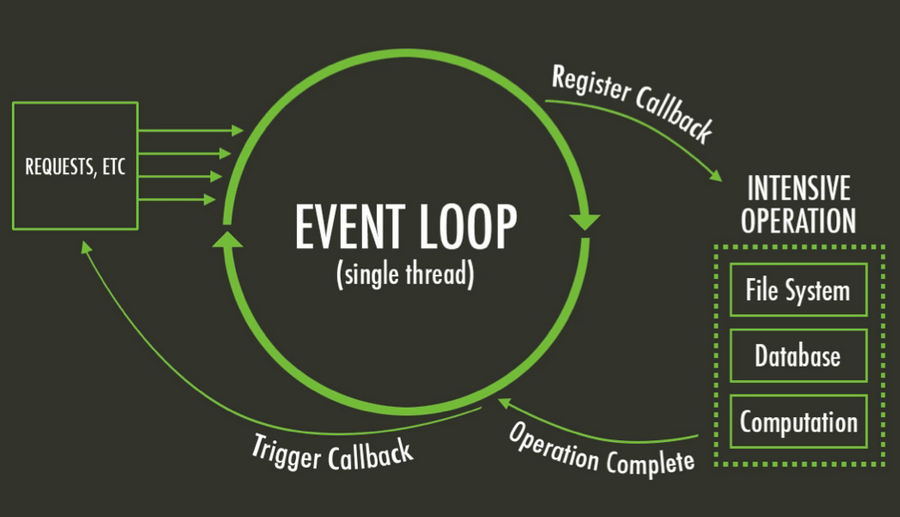
\includegraphics[width=15cm]{graphs/node_eventloop.png} \caption{Sistema de eventos en NodeJS \cite{nodejs}}
\label{fig:nodeEvent}
\end{figure}

\subsubsection{Funcionamiento}
Node ejecuta V8 JavaScript, es decir JavaScript del lado del servidor. El motor V8 JavaScript es el motor JavaScript subyacente que Google usa con su navegador Chrome. Un motor JavaScript interpreta el código y lo ejecuta. Con el V8, Google creó un intérprete ultra-rápido escrito en C++ con otro aspecto único: cualquiera puede descargar el motor e incorporarlo a cualquier aplicación que desee. Gracias a que este no está restringido a ejecutarse en un navegador, Node aprovechó está faceta y le dio otro propósito para así usarlo en el servidor.

\subsubsection{Programación orientada a eventos}
Node utiliza lo que se conoce como modelo de programación orientado por eventos, a diferencia de la programación orientada a objetos que utilizan lenguajes comúnmente usados como Java.
El lado del servidor realmente no es tan diferente del lado del cliente. Es cierto que el usuario no está interactuando con una página web en concreto, ya sea presionando botones o ingresando texto en campos, pero a un nivel superior, están sucediendo eventos. Ejemplos de estos pueden ser una conexión establecida, la recepción de datos a través de dicha conexión, o el hecho de dejar de recibir datos por esa conexión.
¿Por qué este tipo de configuración es ideal para Node? JavaScript es un gran lenguaje para la programación orientada a eventos, ya que permite funciones y cierres anónimos, y más importante, la sintaxis es similar para casi cualquier persona que haya programado en Java o C++. Las funciones de retrollamada o \tit{callbacks} que se llaman y ejecutan cuando ocurre un evento pueden escribirse en el mismo punto en el que el evento es capturado, con lo cual facilita la programación y el mantenimiento de estas. No existen arquitecturas complicadas orientadas a objetos ni tampoco interfaces, simplemente esperar por un evento y escribir una retrollamada qué contendrá las tareas a realizar cuando dicho evento ocurra.

\subsubsection{Módulos Node}
En NodeJS el código se organiza por medio de módulos, que son como los paquetes o librerías de otros lenguajes como Java. Por su parte, NPM es el nombre del gestor de paquetes que usamos en NodeJS.

NPM es bastante similar a los gestores de paquetes de Linux (apt-get en Ubuntu) y se puede entender como una forma de administrar módulos que deseamos tener instalados, distribuir los paquetes y agregar dependencias a nuestros programas.

El gestor de paquetes NPM, no obstante, difiere ligeramente de otros gestores de paquetes conocidos, ya que los instala localmente en los proyectos. Es decir, al descargarse un módulo, este se agrega a un proyecto local, que es el que lo tendrá disponible para incluir.

Cabe decir que también existe la posibilidad de instalar los paquetes de manera global en nuestro sistema, los cuales facilitan tareas relacionadas con el sistema operativo. Estos paquetes, una vez instalados, se convierten en comandos disponibles en el terminal, con los que se pueden realizar multitud de tareas. Ejemplos de este tipo de módulos son Bower, Grunt o Gulp.

\chapterend{}